\chapter{Landasan Teori}
\label{sec:landasanteori}

\section{Odoo}
\label{sec:odoo}

Odoo adalah aplikasi \textit{Enterprise Resource Planning} (ERP) open source adalah web aplikasi yang dibangun menggunakan bahasa pemrograman Python, XML, dan JavaScript dan menggunakan PostgreSQL sebagai database management sistemnya.  Odoo merupakan sebuah sistem atau software manajemen open source, yang sangat mudah untuk digunakan. Bentuk dari sistem Odoo ini terdapat berbagai macam, diantaranya adalah berbasis web, desktop serta mobile. Selain itu, software ini memiliki banyak kelebihan seperti didukung oleh banyak komunitas, modul yang lengkap dan terintegrasi, pemasangan yang mudah, dan juga biaya yang terjangkau. Aplikasi bisnis yang terintegrasi dalam Odoo berbentuk modul-modul yang siap untuk diunduh dan digunakan dan sebagian besar bisa didapatkan secara gratis \cite{suminten}.

\subsection{Struktur Direktori}
\label{sec:strukturDirektori}
Pada bagian ini akan dibahas struktur direktori pada Odoo, salah satunya adalah Odoo Modul. Modul Odoo adalah perpaduan antara server dan client yang disatukan dalam satu modul yang dapat diakses atau dimuat melalui database. Modul Odoo adalah kumpulan fungsi dan data yang dapat melakukan berbagai hal dan tujuan. Segala sesuatu pada Odoo dimulai pada suatu modul. Penggunaan modul ini sendiri dapat dilakukan secara bebas sesuai dengan kebutuhan yang diperlukan oleh pengguna. Modul utama yang dapat dilihat oleh pengguna dapat berbentuk sebagai Aplikasi, namun sebagian besar modul bukan hanya Aplikasi. Modul juga dapat disebut sebagai addons dan direktori tempat server Odoo dapat menemukan addons yang dibuat oleh developer dapat dilihat pada folder addonspath \footnote{Modul Odoo \url{https://www.odoo.com/documentation/16.0/developer/tutorials/getting_started/01_architecture.html}}. 

Komposisi pada modul dapat berisi sejumlah elemen, terdapat beberapa element yaitu:

\begin{enumerate}
	\item \textit{Business Objects} \\
	Objek bisnis dideklarasikan sebagai kelas Python. Objek bisnis ini secara otomatis dipetakan ke kolom basis data.
	\item \textit{Object Views} \\
	Menampilkan tampilan \textit{User Interface} (UI).
	\item \textit{Data Files} \\
	File XML atau CSV yang mendeklarasikan model data, beberapa contoh diantaranya adalah laporan, aturan keamanan, dan data demo.
	\item \textit{Web Controllers} \\
	Menanganin permintaan dari dari web browser.
	\item \textit{Static Web Data}
	File gambar, CSS, atau JavaScript yang digunakan oleh antarmuka website.
\end{enumerate}

Struktur modul pada Odoo adalah direktori di dalam direktori modul. Direktori modul ditentukan dengan menggunakan opsi pada bagian folder --addons-path, dan modul Odoo dideklarasikan menggunakan file manifest. Ketika suatu modul akan dibuat maka modul tersebut diatur sebagai sebuah file python dengan file init.py, file ini berisi instruksi impor untuk berbagai file python di dalam modul. Berikut adalah contoh direktori sebuah modul Odoo.

\begin{figure}[H]
	\centering
	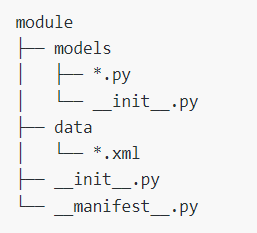
\includegraphics[scale=1]{Gambar/modulOdoo.png}
	\caption{Contoh Direktori Modul Odoo} 
	\label{fig:modulOdoo}
\end{figure}

\subsection{Instalasi}
\label{sec:instalasi}
Pada skripsi ini Odoo akan dinstalasi menggunakan cara \textit{Source Install}, proses instalasi ini bukan hanya sekedar install odoo dan menggunakannya langsung dari sumber website Odoo. Proses instalasi ini lebih nyaman digunakan oleh penulis karena untuk mengembangkan modul akan lebih mudah untuk diakses dibandingkan menggunakan instalasi yang sudah paket.
Dalam proses penggunaan Odoo, akan lebih mudah untuk menjalankan dan menghentikan Odoo, sehingga terlihat lebih flexibel dibandingkan menggunakan instalasi yang sudah satu paket dan juga memungkinkan pengaturan menggunakan baris perintah, tanpa harus mengubah file konfigurasi pada Odoo. Secara tidak langsung, proses intalasi ini memberikan kontrol yang lebih besar atas pengaturan sistem dan memungkinkan untuk lebih mudah menyimpan dan menjalankan beberapa versi Odoo secara bersamaan. \footnote{Instalasi Odoo \url{https://www.odoo.com/documentation/16.0/administration/install/install.html}} Terdapat beberapa cara mengenai cara untuk melakukan instalasi Odoo 16, yaitu:
\begin{enumerate}
	\item Online \\
	Instalasi secara online adalah cara termudah untuk menggunakan Odoo dalam membangun sistem produksi.
	\item Package installer \\
	Instalasi secara \textit{package installer} adalah cara yang sempurna untuk menguji Odoo, mengembangkan modul, dan dapat digunakan untuk penggunaan produksi jangka panjang dengan intalasi tambahan dan \textit{maintenance} tambahan.
	\item Install source \\
	Instalasi secara \textit{install source} adalah cara install odoo dengan memberikan fleksibilitas yang lebih besar, contohnya adalah memungkinkan beberapa versi Odoo berjalan di sistem yang sama, baik untuk mengembangkan modul. Instalasi source ini adalah cara install Odoo yang akan digunakan pada skripsi ini.
	\item Docker \\
	Instalasi Docker dapat digunakan untuk instalasi Odoo karena pengembangan aplikasi yang cepat, mudah, dan portabel.
\end{enumerate}

Pada proses instalasi secara source, terdapat dua cara untuk mengunduh kode Odoo, yaitu melalui arsip zip atau menggunakan git. Dalam penulisan skripsi ini akan dilakukan instalasi Odoo menggunakan git dalam mendapatkan kode Odoo. Tahapan pertama dalam instalasi ini adalah Git harus sudah terinstal di perangkat yang akan digunakan, dan developer harus memiliki pengetahuan dasar dalam proses penggunaan Git. Selanjutnya, untuk mengkloning repositori Git, developer harus memilih salah satu cara antara mengkloning dengan HTTPS atau SSH.

\begin{figure}[H]
	\centering
	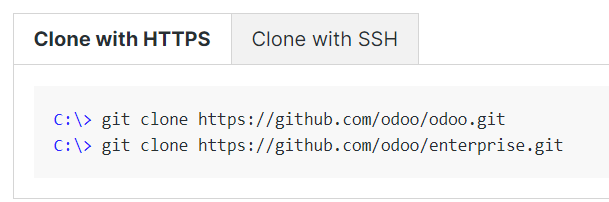
\includegraphics[scale=0.7]{Gambar/clone.png}
	\caption{Contoh Intalasi Source menggunakan Git} 
	\label{fig:clonegit}
\end{figure}

Tahap selanjutnya adalah mempersiapkan Python, sistem Odoo membutuhkan minimal versi 3.7 atau lebih, apabila Python sudah pernah diinstal, maka harus dilakukan pemerikasaan apakah Python sudah menggunakan versi 3.7 atau belum, karena versi dibawah 3.7 tidak cocok untuk instalasi Odoo. Cara yang dapat dilakukan untuk melihat versi Python dapat menggunakan cara sebagai berikut melalui \textit{command prompt} (CMD).

\begin{figure}[H]
	\centering
	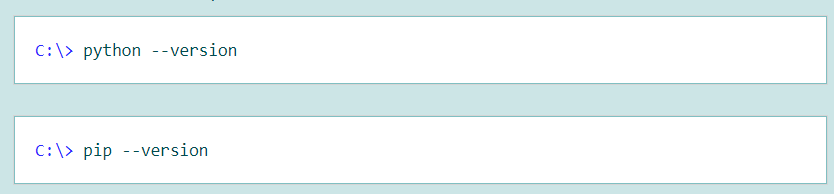
\includegraphics[scale=0.7]{Gambar/python.png}
	\caption{Contoh Melihat Versi Python dan Pip} 
	\label{fig:pip}
\end{figure}

Tahap selanjutnya adalah mempersiapkan PostgreSQL. Odoo menggunakan PostgreSQL sebagai sistem manajemen basis data. Pengguna dapat mengunduh dan instal PostgreSQL minimal versi 12.0 atau yang lebih terbaru. Pada proses intalasi PostgreSQL, pengaturan awal pengguna PostgreSQL adalah postgres, namun Odoo menyarankan untuk tidak menghubungkan database ke postgres, sehingga pengguna diharuskan untuk membuat user atau role baru di PostgreSQL. Berikut tahapan yang harus dilakukan ketika akan melakukan instalasi PostgreSQL:

\begin{enumerate}
	\item Tambahkan direktori bin PostgreSQL (secara pengaturan awal tersimpan di C:-Program Files-PostgreSQL-<version>-bin) ke PATH perangkat yang digunakan. Pada penulisan skripsi ini, PostgreSQL yang digunakan adalah versi 15, sehingga penulisan pada path adalah (C:-Program Files-PostgreSQL-15-bin).
	\item Buat baru nama pengguna postgres dengan kata sandi melalui pgAdmin GUI.
		\begin{itemize}
			\item Buka program pgAdmin.
			\item Klik dua kali pada bagian menu server untuk membuat koneksi.
			\item Pilih bagian menu Objek lalu buat nama untuk login atau role.
			\item Input nama di kolom nama (misalkan: odoo).
			\item Pilih bagian \textit{definition} lalu input password.
			\item Pilih bagian \textit{privileges} lalu pilih bagian dapat login dan buat database.
		\end{itemize}
\end{enumerate}

\begin{figure}[H]
	\centering
	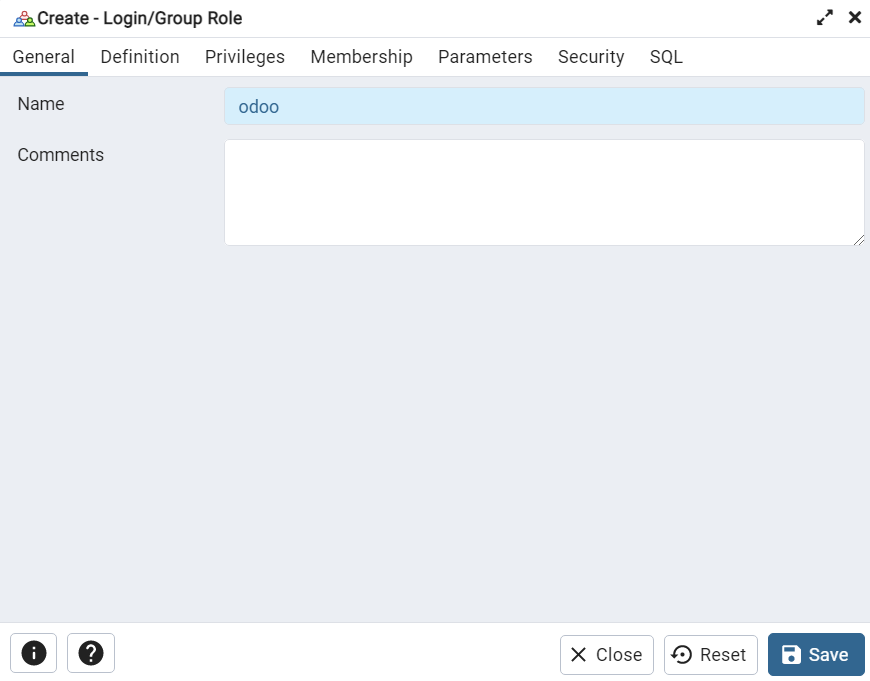
\includegraphics[scale=0.7]{Gambar/psql.png}
	\caption{Contoh Membuat Database pada PostgreSQL} 
	\label{fig:psql}
\end{figure}

Tahapan selanjutnya yang perlu dilakukan dalam instalasi Odoo adalah melakukan beberapa instalasi tambahan. Sebelum proses ini dilakukan, pengguna harus mengunduh dan menginstal \textit{Build Tools for Visual Studio}, lalu pilih C++ build tools pada bagian tab Workloads dan lakukan proses instalasi. Setelah proses ini dilakukan, pengguna harus membuka \textit{command prompt} (CMD) dan melakukan beberapa proses seperti pada gambar berikut:

\begin{figure}[H]
	\centering
	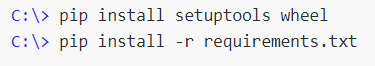
\includegraphics[scale=1]{Gambar/setupOdoo.png}
	\caption{Contoh Perintah untuk Melakukan Proses Instalasi Tambahan} 
	\label{fig:setupOdoo}
\end{figure}

Tahapan terakhir yaitu proses menjalankan Odoo, pada penulisan skripsi ini, penulis menggunakan aplikasi PyCharm, gunakan aplikasi ini untuk membuka folder yang sudah berhasil di clone lalu membukanya melalui PyCharm, setelah itu lakukan beberapa perubahan pada environment, sehingga server Odoo dapat dijalankan. Berikut contoh perubahan pada environment pada PyCharm:

\begin{figure}[H]
	\centering
	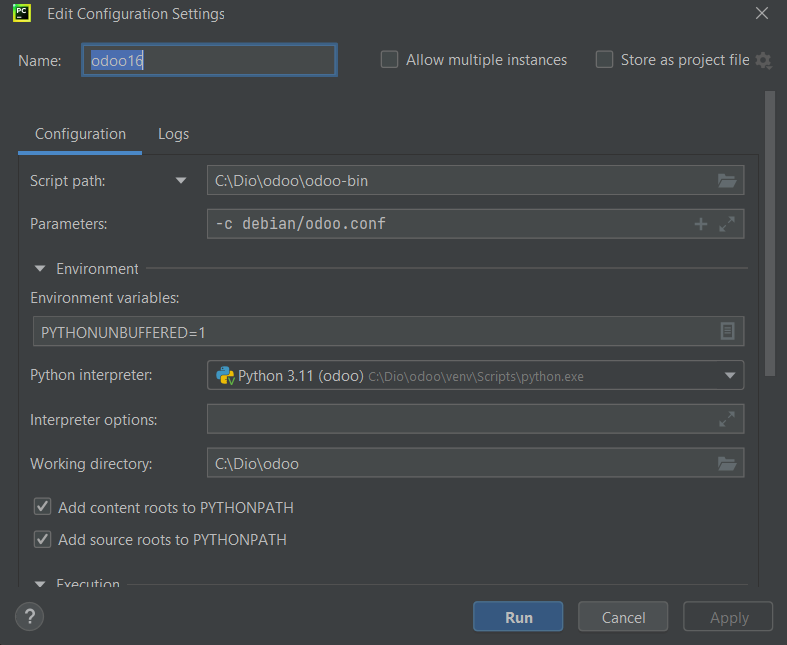
\includegraphics[scale=0.7]{Gambar/pycharm.png}
	\caption{Contoh Perubahan Pengaturan pada PyCharm} 
	\label{fig:pycharm}
\end{figure}

Setelah server berhasil dijalankan (log INFO odoo.modules.loading: Modul sedang diproses), secara pengaturan awal, halaman untuk membuka website awal Odoo adalah \url{http://localhost:8069} yang dilakukan di browser web dan masuk dengan akun admin.

\begin{figure}[H]
	\centering
	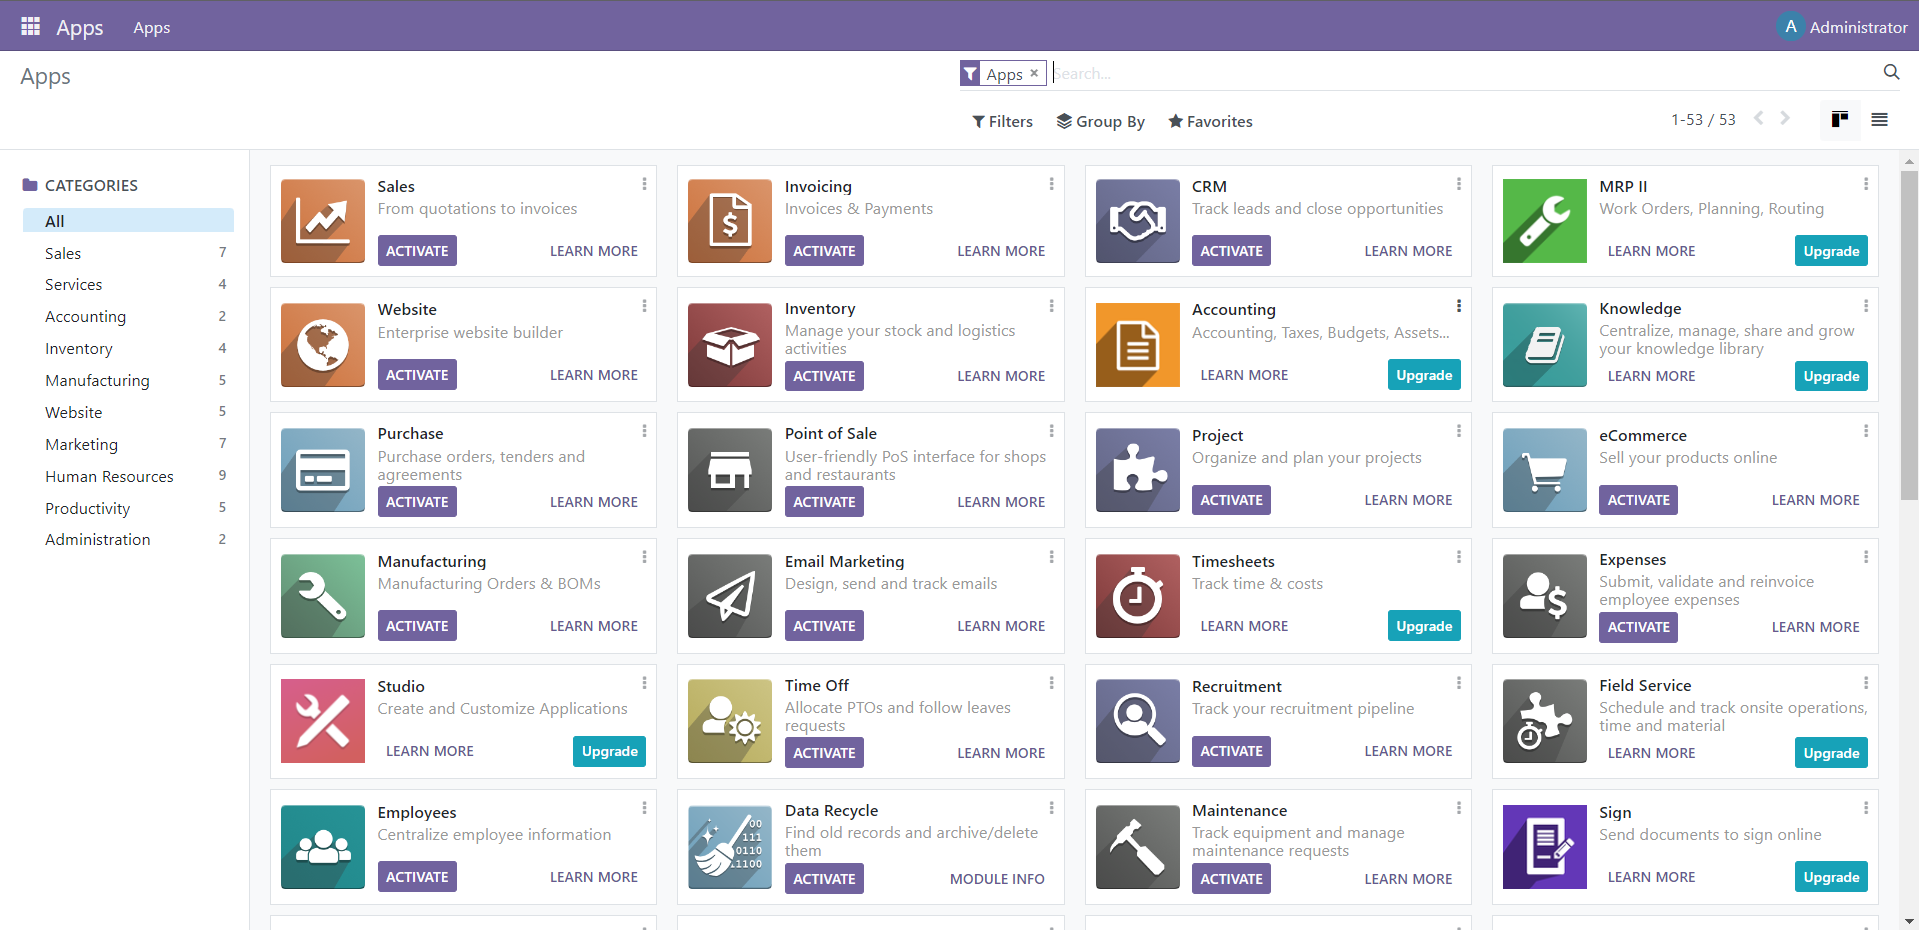
\includegraphics[scale=0.4]{Gambar/halamanOdoo.png}
	\caption{Contoh Halaman Odoo} 
	\label{fig:halamanOdoo}
\end{figure}

\section{Sistem Informasi Manajemen Umat (SIMU)}
\label{sec:simu}
Sistem Informasi Manajemen Umat (SIMU) adalah aplikasi milik Keuskupan Bandung, aplikasi ini bertujuan untuk mencatat data umat dan dinamikanya (contohnya adalah sakramen). Keuskupan Bandung memiliki sekitar 108.000 umat, plus umat Sibolga.
 
\subsection{Umat Baru}
\label{sec:umatBaru}
Cara kerja sistem ini adalah apabila terdapat ada umat baru yang sebelumnya tidak tercatat di SIMU, maka admin akan memberikan print-out dari Formulir Data Umat kepada yang bersangkutan. Apabila keluarga belum tercatat di SIMU, maka admin akan memberikan print-out dari Formulir Keluarga Katolik atau Rumah Tangga Katolik untuk diisi. Formulir ini biasanya dimiliki oleh paroki masing-masing. Apabila tidak tersedia, maka umat dapat menghubungi admin keuskupan untuk mendapatkannya, dalam proses ini diharapkan umat dapat mengisi formulir dengan lengkap dan benar lalu dikembalikan ke sekretariat paroki. 

Proses input data akan dilakukan oleh admin dengan cara admin memilih menu Umat, lalu admin akan klik tombol "Buat" di kiri atas, lalu data yang sudah ada akan diisikan ke dalam formulir, kemudian admin akan menyimpannya, dan untuk penulisan nama umat, umat diharapkan menuliskannya menggunakan huruf kapital secara keseluruhan. Apabila umat memiliki foto untuk dimasukan, umat dapat memasukan foto (opsional), semua hal tadi dapat diulangi oleh admin untuk seluruh umat baru yang akan dimasukkan datanya ke dalam sistem.

\begin{enumerate}
	\item Khusus Bayi \\
	Apabila bayi yang baru lahir, umat diharapkan mengisikan "Belum Beragama" pada kolom agama, hal tersebut bertujuan supaya saat di masa depan akan menerima sakramen baptis, bayi tersebut muncul di daftar pilihan umat yang belum menjadi Katolik.
	\item Umat Ganda \\
	Apabila sudah ada sistem deteksi umat ganda, admin diperlukan untuk memastikan bahwa umat belum pernah masuk sistem SIMU sebelumnya.
\end{enumerate}

\begin{figure}[H]
	\centering
	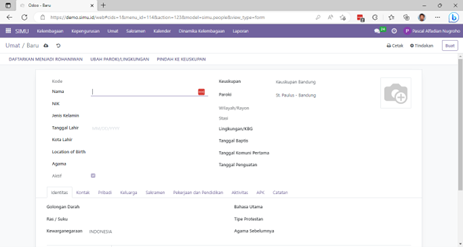
\includegraphics[scale=1]{Gambar/formSimu.png}
	\caption{Contoh Formulir SIMU} 
	\label{fig:formSimu}
\end{figure}

\subsection{Umat Pindah dari atau ke Paroki atau Lingkungan Lain}
\label{sec:umatPindah}

\begin{enumerate}
	\item Seluruh Anggota Keluarga \\
	Untuk memindahkan seluruh anggota keluarga ke paroki atau lingkungan baru, diperlukan prosedur sebagai berikut:
	\begin{itemize}
		\item Admin menari kepala keluarga dari keluarga katolik tersebut, kemudian klik “Pindah Paroki / Lingkungan”.
		\item Admin memastikan seluruh dokumen sudah diverifikasi (KTP, Surat Baptis, Surat Konfirmasi dari Ketua Lingkungan), lalu admin menekan klik seluruh checkbox yang disediakan, termasuk “Pindahkan seluruh anggota keluarga”. Klik “Simpan” untuk menyimpan.
		\item Admin mencari Keluarga Katolik dari umat tersebut. Setelah ditemukan, admin menekan klik Edit, dan sesuaikan kolom Paroki dan Lingkungan sesuai perubahan pada langkah sebelumnya.
	\end{itemize}
	\item Salah Satu Anggota Keluarga \\
	Untuk melakukan perpindahan umat sebagai salah satu anggota keluarga, diperlukan prosedur sebagai berikut:
	\begin{itemize}
		\item Admin mencari umat yang bersangkutan.
		\item Admin melakukan klik pada kolom “Paroki” dan atau “Lingkungan/KB”, dan mengisikan nilainya dengan paroki tujuan.
		\item Jika umat tersebut berpindah karena menikah, maka umat tersebut harus dicabut dari keluarga yang lama dan dibuatkan atau dipindah ke keluarga baru, dengan cara admin melakukan edit, dan hapus umat tersebut dari keluarga tersebut melalui tab Anggota Keluarga, lalu admin membuat keluarga katolik baru melalui menu Umat dan mendaftarkan kedua anggota yang baru saja menikah (cukup satu keluarga per pasangan yang menikah).
	\end{itemize}
\end{enumerate}

\subsection{Umat Masuk dari Keuskupan Lain}
\label{sec:umatMasuk}
Dari Keuskupan yang Menggunakan BIDUK:
\begin{enumerate}
	\item Umat melapor kepada admin SIMU paroki setempat
	\item Admin Paroki SIMU berkoordinasi dengan admin SIMU Keuskupan melakukan permintaan atau request untuk menarik data umat yang bersangkutan dari BIDUK.
	\item Admin SIMU Keuskupan masuk ke menu Catat Umat Masuk dan mengisikan data umat baru tersebut.
	\item Admin BIDUK menerima permohonan tarik data.
	\item Admin BIDUK mengonfirmasi perpindahan keluar kepada admin paroki SIMU tentang keberadaan umat/keluarga yang dimaksud
\end{enumerate}

\subsection{Umat Keluar ke Keuskupan Lain}
\label{sec:umatKeluar}
Menuju Keuskupan yang Menggunakan BIDUK, prasyarat dari proses ini adalah umat sudah berpindah secara tetap di paroki tujuan, langkah-langkahnya adalah sebagai berikut:
\begin{enumerate}
	\item Umat melapor kepada admin BIDUK paroki setempat
	\item Admin BIDUK melakukan permintaan atau request untuk menarik data umat yang bersangkutan dari SIMU
	\item Admin SIMU menerima permohonan tarik data pada menu Mutasi Antar-Keuskupan Umat Keluar
	\item Admin SIMU mengonfirmasi perpindahan keluar kepada admin paroki SIMU tentang keberadaan umat atau keluarga yang dimaksud.
	\item Apabila perpindahan telah dikonfirmasi, admin SIMU menekan tombol “Setuju” pada permohonan mutasi tersebut.
	\item SIMU akan otomatis mengirimkan data umat atau keluarga yang berpindah ke BIDUK, dan pada SIMU sendiri umat tersebut akan diset sebagain “non-aktif”.
\end{enumerate}

Menuju Keuskupan Lain, pada prosedur ini tidak perlu menunggu umat yang bersangkutan untuk dikonfirmasi di keuskupan tujuan. langkah-langkahnya adalah sebagai berikut:
\begin{enumerate}
	\item Umat melapor kepada admin paroki setempat
	\item Admin Paroki berkoordinasi dengan admin Keuskupan melakukan permintaan atau request untuk menarik data umat yang bersangkutan dari BIDUK
	\item Admin Keuskupan masuk ke Umat tersebut dan klik Pindah ke Keuskupan
	\item Admin Keuskupan mengisi data yang diminta, dan menekan tombol “Simpan”.
\end{enumerate}

\subsection{Data Umat dan/atau Keluarga Berubah}
\label{sec:dataBerubah}
Admin akan mencetak terlebih dahulu Formulir Data Umat dan Formulir Keluarga Katolik atau Rumah Tangga Katolik yang sudah terisi data SIMU, sehingga umat hanya perlu mengoreksi informasi yang perlu diubah tanpa harus menuliskan ulang semuanya kembali. Setelah umat mengembalikan formulir yang sudah dikoreksi, admin akan melakukan perubahan data pada SIMU, dengan cara mencari kembali umat yang bersangkutan, dan memilih tombol Edit. Admin akan memperbaharui data-data yang berubah, kemudian admin akan menekan tombol “Simpan” untuk menyimpan perubahan.

\subsection{Umat Dibaptis}
\label{sec:umatDibaptis}
Umat yang dibaptis harus sudah tercatat sebelumnya di SIMU. Apabila belum terdaftar maka:

\begin{enumerate}
	\item Terdapat kemungkinan umat tersebut sudah didaftarkan di paroki lain. Dalam hal ini, umat harus berkoordinasi dengan paroki di mana umat tersebut berada.
	\item Jika yakin bahwa umat tersebut belum terdaftar di SIMU, admin melakukan prosedur Umat Baru.
\end{enumerate}

Persyaratan untuk melakukan baptis adalah umat yang akan dibaptis perlu melengkapi persyaratan seperti akte kelahiran, formulir calon baptis yang sudah diisi, dan sebagainya. Untuk setiap persyaratan yang telah dipenuhi, admin memberikan tanda centang pada tab “Persyaratan” (dengan sebelumnya membuka entri sakramen tersebut). Dalam proses baptis, calon baptis atau orang tua calon baptis juga perlu mendapatkan pendampingan. Jika pendampingan sudah selesai, umat akan melakukan “Edit” kembali entri yang bersangkutan, masuk ke tab “Pendampingan”, dan isikan tanggal kelulusan. Jika tanggal kelulusan sudah diisi, dan persyaratan lengkap, maka status akan bergerak maju menjadi “Persyaratan Terpenuhi”.
Setelah proses materalisasi dilakukan, tahapan selanjutnya yang terakhir adalah surat-surat, setelah surat dicetak, belum tentu bisa langsung diambil oleh umat yang bersangkutan. Begitupun status di SIMU, di mana surat belum terambil. 

\section{Design untuk Aplikasi Mobile}
\label{sec:designMobility}
Perangkat seluler (smartphone), tablet, game console telah menjadi hal yang umum di dunia komputasi. Desain seluler membuat tata letak estetika antarmuka pengguna. Desain seluler biasa dilakukan oleh software engineers, graphic designers, content developers, security specialists, dan semua orang yang tergabung dalam pembuatan model design. Desain sangatlah penting karena memungkinkan suatu model yang dibuat dapat meningkat nilai kualitasnya. Salah satu contohnya adalah website. Website adalah sekumpulan halaman yang terdiri dari beberapa laman yang berisi informasi dalam bentuk data digital baik berupa text, gambar, video, audio, dan animasi lainnya yang disediakan melalui jalur koneksi internet. Untuk membangun sebuah halaman website dibutuhkan sebuah bahasa pemrograman yang lebih dikenal dengan sebutan web scripting. \cite{batubara2015perancangan}

\subsection{Pertimbangan Teknis}
\label{sec:teknis}
Pertimbangan teknis yang dilakukan untuk menurunkan biaya yang sangat rendah pada kapabilitas menambahkan web pada perangkat sehari-hari seperti ponsel, kamera, dan tv dapat mengubah cara orang mengakses informasi dan menggunakan layanan jaringan. Berikut merupakan beberapa pertimbangan teknis yang harus ditangani oleh aplikasi mobile: 

\begin{enumerate}
	\item Berbagai platform perangkat lunak dan keras \\
	Tidak bisa untuk produk yang berjalan diberbagai platform, karena terdapat perbedaan perangkat lunak dan keras sehingga banyak perbedaan diantara perangkat yang akan digunakan, dan akan membutuhkan waktu dan uang yang cukup mahal
	\item Terlalu banyak frameworks dan bahasa pemograman \\
	Banyaknya bahasa pemograman dan frameworks yang digunakan membuat banyak perbedaan antara setiap perangkat mobile.
	\item Terdapat banyak peraturan pada tempat publish aplikasi \\
	Setiap platform memiliki toko aplikasi dan standarnya sendiri untuk menerima aplikasi yang dibuat. Sehingga setiap aplikasi mobile yang dibuat harus mengikuti setiap peraturan dan standar yang telah ada.
	\item Siklus Aplikasi Mobile \\
	Pada siklus pengembangan aplikasi mobile, waktu yang dibutuhkan cukup lama dalam proses pembuatannya, namun pada akhirnya pasar persaingan aplikasi ini sangatlah cepat, sehingga apabila aplikasi tidak berkembang, maka aplikasi tersebut sudah dipastikan kalah oleh aplikasi lain yang terus bermunculan.
\end{enumerate}

\subsection{User Interface Design}
\label{sec:ui}
Pengguna perangkat seluler berharap apabila mereka menggunakan aplikasi mobile, waktu belajar minimal yang diperlukan untuk mempelajari aplikasi tersebut diharapkan sangatlah cepat, oleh karena itu desainer aplikasi mobile harus bekerja keras dalam membuat suatu aplikasi. Berikut merupakan beberapa pertimbangan yang harus dilakukan dalam membuat \textit{user interface design} pada aplikasi mobile:

\begin{enumerate}
	\item Menentukan brand pokok dari produk tersebut, sehingga terdapat perbedaan dengan produk dari merk pesaing.
	\item Fokus portofolio produk, menargetkan produk apakah untuk plafform android atau ios, karena jumlah pengguna platform tersebut tidaklah sama.
	\item Mengoptimalkan kecepatan dan kemampuan dari aplikasi yang dibuat, karena pengguna tidak mau banyak menunggu.
	\item Tentukan ukuran dan scaling untuk produk yang akan dibuat, sehingga ketika menampilkan sesuatu tidaklah terlalu besar atau kecil.
	\item Keahlian untuk melakukan design antarmuka harus sangat tinggi, karena untuk tata letak, animasi, grafik dibutuhkan keahlian khusus. 
\end{enumerate}

\subsection{Kesalahan Design Aplikasi Mobile}
\label{sec:kesalahanUI}
Berikut merupakan beberapa kesalahan yang terdapat pada design aplikasi mobile:
\begin{enumerate}
	\item Terlalu banyak fitur, hindari menambahkan banyak fitur yang kurang bermanfaat, karena hal tersebut akan mengurangi nilai keindahan, cukup sederhana namun bisa bersaing di pasaran.
	\item Kurang konsisten, tentukan suatu standar pada produk aplikasi mobile yang akan dibuat, sehingga aplikasi yang akan dibuat memiliki patokan dan menghindari produk menjadi kurang konsisten.
	\item Lag atau bisa dibilang kurang cepat dalam membuka atau melakukan sesuatu, hal seperti ini membuat pengguna menjadi banyak menunggu sehingga hanya membuang-buang waktu.
	\item Design yang berlebihan, pemilihan warna, gambar, animasi, ataupun tema menjadi masalah yang penting, apabila produk tersebut memiliki design yang berlebihan, maka pengguna akan merasa tidak nyaman dengan tampilan yang ditampilkan.
	\item Bertele-tele, aplikasi yang dibuat tidak sempat ditest, sehingga saat penggunaan aplikasi tersebut, banyak menu atau pilihan yang tidak berguna, sehingga tujuan yang akan dicapai oleh aplikasi tersebut menjadi hilang atau lama untuk tercapai.
\end{enumerate}

\cite{pressman2019software}

\section{QR Code}
QR Code, kependekan dari Quick Response Code, merupakan gambar dua dimensi yang memiliki kemampuan untuk menyimpan data. QR Code biasa digunakan untuk menyimpan data berupa teks, baik itu numerik, alfanumerik, maupun kode biner. QR Code banyak digunakan untuk keperluan komersil biasanya berisi link url ke alamat tertentu atau sekedar teks berisi iklan, promosi, dan lain-lain. QR Code adalah image dua dimensi yang merepresentasikan suatu data, terutama data berbentuk teks. QR Code merupakan evolusi dari barcode yang awalnya satu dimensi menjadi dua dimensi. QR Code memiliki kemampuan menyimpan data yang
lebih jauh besar daripada barcode.

Versi simbol QR Code berkisar dari versi 1 sampai dengan Versi 40. Setiap versi memiliki konfigurasi modul atau jumlah modul yang berbeda, modul mengacu pada titik hitam dan putih yang membentuk QR Code.
Konfigurasi modul ini dapat dilihat pada jumlah modul yang terdapat dalam simbol, biasa dimulai dengan versi 1 (modul 21 × 21) hingga versi 40 (modul 177 × 177). Setiap nomor versi yang lebih tinggi terdiri dari 4 modul tambahan per sisi. \footnote{Versi Simbol QR Code \url{https://www.qrcode.com/en/about/version.html}}

\begin{figure}[H]
	\centering
	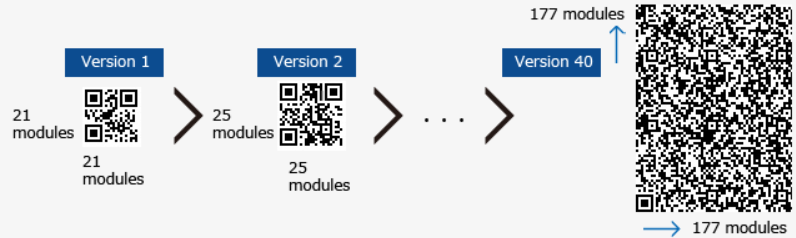
\includegraphics[scale=1]{Gambar/versiQR.png}
	\caption{Contoh Versi QR Code} 
	\label{fig:versiQR}
\end{figure}

Pada setiap versi simbol QR Code memiliki kapasitas data maksimum yang berbeda, tergantung dengan dengan jumlah data, jenis karakter, dan tingkat koreksi kesalahan. Oleh karena itu, seiring bertambahnya jumlah data, semakin banyak pula modul yang dibutuhkan untuk menyusun QR Code, sehingga menghasilkan simbol QR Code yang lebih besar.

Titik untuk mengukur ukuran sebenarnya dari simbol QR Code tergantung pada ukuran milimeter modul (satu area persegi yang terdiri dari QR Code) yang akan dicetak. Semakin besar modulnya, semakin stabil dan mudah dibaca dengan pemindai Kode QR Code. Namun dikarenakan ukuran simbol QR Code semakin besar, area pencetakan yang lebih besar akan diperlukan. Oleh karena itu, perlu untuk menentukan ukuran modul dari setiap aplikasi setelah mempertimbangkan semua faktor yang relevan. Namun tetap disarankan agar simbol QR Code dicetak sebesar mungkin dalam area pencetakan yang tersedia.

\begin{figure}[H]
	\centering
	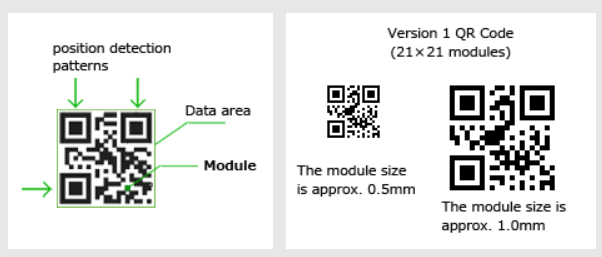
\includegraphics[scale=1]{Gambar/modulSize.png}
	\caption{Contoh Modul QR Code} 
	\label{fig:modulSize}
\end{figure}

\subsection{Masalah pada Mempindai QR Code}
\label{sec:masalahQR}
QR Code dapat dibaca dengan mudah apabila QR Code yang dibuat mengikuti standar QR Code dan harus dicetak dengan jelas. Oleh karena itu QR Code yang tidak mengikuti standar dan tidak jelas gambarnya, sudah dipastikan tidak dapat dibaca dengan jenis pemindai dan ponsel tertentu. Berikut contoh QR Code yang menyebabkan masalah dalam proses pemindaian QR Code:

\begin{enumerate}
	\item QR Code yang modulnya terdistorsi, yang dimaksud disini adalah ketika QR Code diperbesar atau diperkecil menggunakan suatu aplikasi, maka QR Code tidak bisa dibaca atau dipindai.
	\begin{figure}[H]
		\centering
		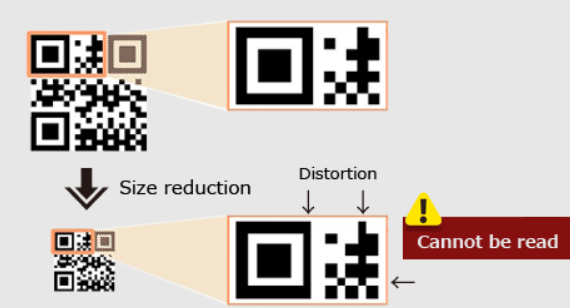
\includegraphics[scale=1]{Gambar/qrDistro.png}
		\caption{Contoh QR Code yang Terdistorsi} 
		\label{fig:qrDistro}
	\end{figure}
	
	\item QR Code yang terdapat huruf atau gambar yang mengelilingi QR Code tersebut, hal ini menyebabkan camera atau alat scan menjadi sulit fokus terhadap modul QR Code.
	\begin{figure}[H]
		\centering
		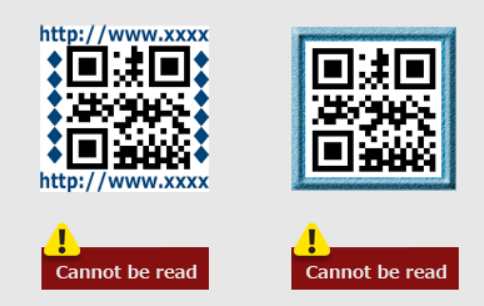
\includegraphics[scale=1]{Gambar/qrGambar.png}
		\caption{Contoh QR Code yang DIkelilingi oleh Gambar atau Huruf} 
		\label{fig:qrGambar}
	\end{figure}
	
	\item QR Code yang tertimpa atau saling tumpang tindih oleh gambar atau huruf, akan menyembabkan kontras area antara warna gelap dan terang sulit untuk dibedakan.
	\begin{figure}[H]
		\centering
		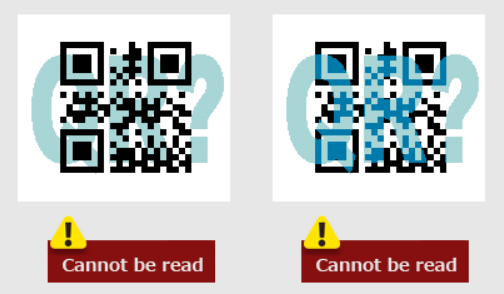
\includegraphics[scale=1]{Gambar/qrTimpa.png}
		\caption{Contoh QR Code yang Tumpang Tindih oleh Gambar atau Huruf} 
		\label{fig:qrTimpa}
	\end{figure}
\end{enumerate}


